% PLDI submission skeleton (ACM acmart, sigplan format).
%
% Build:  ./build.sh           (uses tectonic, which fetches acmart automatically)
% or:     latexmk -pdf main.tex (requires a TeX Live with acmart)
%
% PLDI uses the ACM `acmart` class in `sigplan` format with anonymous review.
\documentclass[sigplan,10pt,review,anonymous]{acmart}
% \documentclass[sigplan,10pt,review]{acmart}

\settopmatter{printfolios=true}
\renewcommand\footnotetextcopyrightpermission[1]{}
\pagestyle{plain}

\usepackage{amsmath,amsthm}
\usepackage{booktabs}
\usepackage{graphicx}
% Per-environment figure selection.  build.sh writes figures/env.tex with a
% \figroot override (e.g. figures/a100/) so a build uses one machine's plots;
% without it we fall back to the shared figures/ directory.
\providecommand{\figroot}{figures/}
\InputIfFileExists{figures/env.tex}{}{}
% Include a generated figure if present, else a placeholder box.
\newcommand{\paperfig}[2]{%
  \IfFileExists{\figroot #1.pdf}%
    {\includegraphics[width=\linewidth]{\figroot #1.pdf}}%
    {\fbox{\parbox[c][2.6cm][c]{0.92\linewidth}{\centering #2\\[2pt]%
     \footnotesize(run \texttt{paper/plots/make\_figures.py})}}}}
\usepackage{tikz}
\usetikzlibrary{arrows.meta,positioning,fit,backgrounds,calc}
\usepackage{subcaption}
\usepackage{fontspec}
% Code font: Fira Code, vendored under src/fonts for a reproducible build.
% Ligatures are disabled so \texttt{} and listings stay literal.
\setmonofont{FiraCode-Regular}[
  Path = fonts/,
  BoldFont = FiraCode-Bold,
  Scale = 0.92,
  Ligatures = NoCommon,
  RawFeature = {-liga,-calt},
]
\usepackage{listings}
\definecolor{codebg}{RGB}{247,247,249}
\definecolor{codekw}{RGB}{30,90,160}
\definecolor{codetype}{RGB}{120,60,150}
\definecolor{codestr}{RGB}{160,70,40}
\definecolor{codecom}{RGB}{110,120,110}
\definecolor{coderule}{RGB}{215,215,222}
\lstdefinestyle{pars}{
  basicstyle=\ttfamily\scriptsize,
  keywordstyle=\color{codekw}\bfseries,
  keywordstyle=[2]\color{codetype},
  commentstyle=\color{codecom}\itshape,
  stringstyle=\color{codestr},
  columns=fullflexible, keepspaces=true, breaklines=true, tabsize=2,
  backgroundcolor=\color{codebg},
  frame=single, framerule=0.3pt, framesep=3pt, rulecolor=\color{coderule},
  aboveskip=6pt, belowskip=3pt, xleftmargin=3pt, framexleftmargin=3pt,
  showstringspaces=false,
  morekeywords={struct,using,template,class,typename,constexpr,auto},
  morekeywords={[2]type_list,seq,alt,opt,star,plus,lit,cls,any,rule,notp,
                lexical_rules,fallback_rules,rules,start,def},
}
\lstset{style=pars,language=C++}

\newtheorem{definition}{Definition}
\newtheorem{proposition}{Proposition}
\newtheorem{theorem}{Theorem}
\newtheorem{lemma}{Lemma}

% Shorthands
\newcommand{\SA}{\mathfrak{S}}
\newcommand{\NBP}{\textsf{NBP}}
\newcommand{\Rone}{R1}
\newcommand{\Rtwo}{R2}
\newcommand{\Rthree}{R3}
\newcommand{\Rfour}{R4}
\newcommand{\Rfive}{R5}
\newcommand{\Rsix}{R6}
\newcommand{\Rseven}{R7}
\newcommand{\shapes}{\mathsf{shape}}
\newcommand{\affine}{\mathit{affine}}
\newcommand{\dyck}{\mathit{dyck}}
\newcommand{\tab}{\mathit{table}}
\newcommand{\code}[1]{\texttt{#1}}

\title{Pars: Compiling Grammars to Data-Parallel Parsers}

\author{Junze Dai}
\author{Xianwei Zhang}
\affiliation{
    \institution{Sun Yat-Sen University} 
    \country{China}
}
\email{dvdbr3o@qq.com}

\begin{document}

\begin{abstract}
Parsing is sequential in its classical formulation, yet state-of-the-art JSON
parsers such as \textsf{simdjson} and \textsf{cuJSON} run an order of magnitude
faster than textbook parsers by exploiting a small set of data-parallel
primitives.  These primitives are usually presented as format-specific tricks
(\textsf{prefix\_xor}, depth-sort bracket matching, \ldots), which makes them
hard to reuse and impossible to derive.

We show that they are instances of a single algebra, the \emph{scan algebra} $\SA$, and that
a grammar can be compiled to a data-parallel parser by a \emph{mechanical
rewrite} of a naive branch program into branchless masked data flow:
a stateful byte recurrence becomes a prefix product in a \emph{transformation
monoid} (a parallel scan), a filter becomes a \emph{compaction}, and the parser
stack becomes a \emph{well-nested reduction}.  Masking is derived from a
compiled automaton, not from the syntactic shape of rules; a specialization is
emitted only when it is provably equivalent to the automaton.

We build a compiler that turns a grammar into a CUDA implementation, and
evaluate it on JSON, CSV, TOML, XML, INI and a C-like language, on two testbeds
(a laptop GPU and an A100 node).  Separating transport from compute, the
generated device-resident scanners match or exceed domain SOTA: on CSV they
reach $3.6\times$ \textsf{simdcsv} on the laptop and $23\times$ on the A100,
and on TOML/INI/XML and C-like---none of which has a SIMD or GPU parser---they
run far ahead of the best CPU parsers.  Adding data movement is decisive: the
host-boundary chunked path is PCIe-limited, staying below \textsf{simdcsv} on
CSV on the laptop while surpassing it on the A100 node, whose shared CPU is the
bottleneck.
\end{abstract}

\maketitle

\section{Introduction}
\label{sec:intro}

Parsing has traditionally been treated as an inherently sequential problem: a
recursive-descent or LR parser consumes bytes left to right, and its control
flow (a stack, lookahead, backtracking) defeats vectorization.  Yet modern
parsers do run fast.  \textsf{simdjson}~\cite{simdjson} scans JSON at gigabytes
per second on a CPU using bit-parallel masks and a prefix scan;
\textsf{cuJSON}~\cite{cujson} runs the same idea on a GPU; \textsf{simdcsv}
does the analogous thing for CSV~\cite{simdcsv}.  The literature, however,
describes these systems as collections of format-specific tricks.  This makes
two questions hard:
\begin{enumerate}
  \item \textbf{Why} do the tricks work, and what is the space of grammars to
        which they apply?
  \item \textbf{How} does one obtain such a parser for a \emph{new} grammar,
        without re-deriving the tricks by hand?
\end{enumerate}

This paper answers both by exhibiting a single algebra, the \emph{scan algebra} $\SA$, and
a compiler built on it.  The key idea is to view fast parsing as
\emph{branch masking}: the branchy scalar program that a grammar suggests is
rewritten into branchless masked data flow.  Concretely, a byte-level
recurrence
\[
  s_{i+1} = T_{c_i}(s_i)
\]
(where $c_i$ is the class of byte $i$) induces, for every byte, a transform
$\tau_i : S \to S$; the running state is therefore the \emph{prefix product}
$\tau_{i-1}\circ\cdots\circ\tau_0$ in the transformation monoid $(S\to S,\circ)$
--- a parallel scan.  For $S=\{0,1\}$ this is the affine recurrence
$x' = (a\wedge x)\oplus b$ whose prefix is exactly
\textsf{simdjson}'s \textsf{prefix\_xor} and \textsf{cuJSON}'s escape scan.
Filtering tokens is a stream compaction; the parser stack, for a well-nested
language, is a depth group-scan plus a sort.

\paragraph{Contributions.}
\begin{itemize}
  \item \textbf{Scan algebra $\SA$} (\S\ref{sec:model}): a small algebra of primitives
        (classification, monoid scan, masked select, compaction, well-nested
        reduction, associative reduction) and a rewrite system that turns a
        naive branch program into branchless data flow.  We characterize the
        grammars to which the rewrite applies (regular rule bodies plus
        visibly-pushdown or associative recursion) and give a cost model that
        separates compute parallelism from data movement.
  \item \textbf{A compiler} (\S\ref{sec:impl}): a shape-free front end that
        compiles each lexical rule to a DFA by Brzozowski derivatives, derives
        masking from the automaton, and emits a per-rule \emph{monoid
        descriptor}.  Backends execute the descriptor as a prefix scan; a
        specialization (affine / doubled / comment) is emitted only when it is
        provably equivalent to the general automaton.
  \item \textbf{An evaluation} (\S\ref{sec:eval}) across seven grammars and
        three throughput tiers, including formats with \emph{no} prior
        SIMD/GPU parser, at multiple input scales.
\end{itemize}

\paragraph{What this is not.}  The scan algebra $\SA$ does not parallelize general CFG
parsing.  Unbounded backtracking and non-well-nested recursion fall outside it
and must be declared as fallbacks.  The algebraic components are classical
(\S\ref{sec:related}); our contribution is their \emph{systematization into a
compiler} and the explicit distinction between compute parallelism and data
movement.

\section{Overview}
\label{sec:overview}

A user writes a grammar as an ordinary C++ type.  The compiler lowers it,
entirely at compile time, to a data-parallel scanner whose structure is fixed by
the scan algebra $\SA$ (Figure~\ref{fig:framework}).  This section gives the intuition; the
formalization follows in \S\ref{sec:model}.

% Framework pipeline diagram (placeholder; may be hand-drawn).
\begin{figure}[t]
\centering
\resizebox{\linewidth}{!}{%
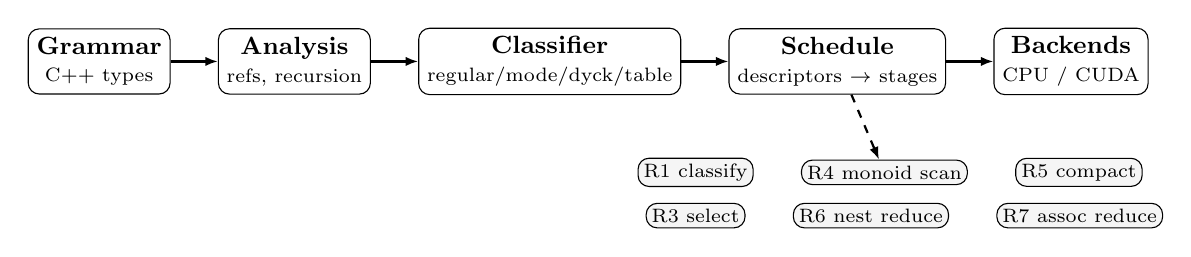
\begin{tikzpicture}[
  node distance=6mm,
  box/.style={draw, rounded corners, align=center, inner sep=3pt, font=\small},
  prim/.style={draw, rounded corners, fill=black!4, align=center, inner sep=2pt, font=\scriptsize},
  ar/.style={-{Latex[length=1.6mm]}, thick}]

\node[box] (g) {\textbf{Grammar}\\[-1pt]\scriptsize C++ types};
\node[box, right=of g] (a) {\textbf{Analysis}\\[-1pt]\scriptsize refs, recursion};
\node[box, right=of a] (c) {\textbf{Classifier}\\[-1pt]\scriptsize regular/mode/dyck/table};
\node[box, right=of c] (s) {\textbf{Schedule}\\[-1pt]\scriptsize descriptors $\to$ stages};
\node[box, right=of s] (b) {\textbf{Backends}\\[-1pt]\scriptsize CPU / CUDA};

\draw[ar] (g) -- (a);
\draw[ar] (a) -- (c);
\draw[ar] (c) -- (s);
\draw[ar] (s) -- (b);

\node[prim, below=8mm of s, xshift=-18mm] (r1) {R1 classify};
\node[prim, right=of r1] (r4) {R4 monoid scan};
\node[prim, right=of r4] (r5) {R5 compact};
\node[prim, below=2mm of r1] (r3) {R3 select};
\node[prim, right=of r3] (r6) {R6 nest reduce};
\node[prim, right=of r6] (r7) {R7 assoc reduce};
\draw[ar, dashed] (s) -- (r4);
\end{tikzpicture}%
}
\caption{The compiler and scan algebra $\SA$.  A grammar is lowered, entirely at
compile time, to a schedule of primitives executed by CPU/CUDA backends.}
\label{fig:framework}
\end{figure}


\paragraph{The surface language.}
The whole user input is one C++ type: rules are tag structs, rule bodies are
type aliases, and there is no run-time grammar object.  Figure~\ref{fig:grammar}
is a JSON fragment.

\begin{figure}[t]
\begin{lstlisting}
struct json_grammar {
  struct value {}; struct string {};
  struct number {}; struct ws {};
  using rules         = type_list<value, string,
                                  number, ws>;
  using lexical_rules = type_list<string, number, ws>;
  using start = value;
  template <class> struct def;
};
template <> struct json_grammar::def<
    json_grammar::string> {
  using type = seq<lit<'"'>,
      star<alt<seq<lit<'\\'>, any>,
               seq<notp<cls<'"','\\'>>, any>>>,
      lit<'"'>>;
};
\end{lstlisting}
\caption{A grammar is a type.  \code{lexical\_rules} marks the rules that mask;
all other rules are classified as structural or recursive by the front end
(automaton + FIRST/LAST + the bracket guard), never by pattern matching.
The full seven-grammar suite ships in the artifact.}
\label{fig:grammar}
\end{figure}

\begin{table}[t]
\centering\small
\caption{Surface constructs and their grammar meaning.}
\label{tab:dsl}
\begin{tabular}{@{}ll@{}}
\toprule
Construct & Grammar meaning \\
\midrule
\code{lit<c>}, \code{cls<c...>}, \code{any} & terminal, byte class, wildcard \\
\code{seq<>}, \code{alt<>} & concatenation, alternation \\
\code{opt<>}, \code{star<>}, \code{plus<>} & Kleene operators \\
\code{rule<T>} & nonterminal reference \\
\code{notp<T>} & negated predicate (lookahead) \\
\code{rules}, \code{start}, \code{def<T>} & rule set, start symbol, body \\
\code{lexical\_rules} & mask these rules \\
\code{fallback\_rules} & opt-out to a fallback backend \\
\bottomrule
\end{tabular}
\end{table}

\paragraph{From a branch program to masked data flow.}
Consider the scalar loop that masks JSON strings:
\begin{lstlisting}
in = esc = false;
for (i = 0; i < n; ++i) {
  c = data[i];
  if (in) {
    if (esc)              esc = false;
    else if (c == '\\')   esc = true;
    else if (c == '"')    in  = false;
  } else {
    if (c == '"')         in  = true;
    else if (structural(c)) emit(i);
  }
}
\end{lstlisting}
Every condition is a predicate on the current byte and a bounded register.  The
rewrite replaces each byte by the state transform it induces and the loop by a
\emph{prefix scan} over the transformation monoid; a branch becomes a masked
select.  For the 1-bit \texttt{in}-flag the transform is affine,
$x'=(a\wedge x)\oplus b$, and its prefix is a single
\textsf{prefix\_xor} over the quote mask once escaped quotes are removed.

\paragraph{Masking from an automaton, not a shape.}
We do not pattern-match rule syntax.  Each lexical rule is compiled to a DFA by
Brzozowski derivatives, and a byte is masked iff the DFA transition it takes is
one that \emph{consumes it as part of an in-progress token}.  This one rule
subsumes prefix-escaped strings, doubled-quote strings, line and block comments,
and multi-mode languages.  Specializations (affine, doubled, comment) are
emitted only when an exhaustive check shows them equivalent to the automaton.

\paragraph{Parsing as well-nested reduction.}
For a well-nested (visibly pushdown) recursion, the stack is replaced by a
depth group-scan plus a sort: depth is the prefix sum over open/close brackets,
and matched pairs are adjacent tokens after a stable sort by depth.  This is
\textsf{cuJSON}'s stack-free matching, derived from the grammar rather than
special-cased.

\paragraph{Boundary, kernels, chunking --- not transfer.}
The framework owns the device boundary: \code{scan\_device} is zero-copy
(input on device, results on device), the \code{scan\_host} adapter is the only
place with bulk transfers, and \code{scan\_chunk} carries the prefix-monoid
state and output offset so chunks can be pipelined.  This separation is what
makes the three throughput tiers of \S\ref{sec:eval} meaningful: a compute
roofline, an on-device number, and a host-boundary number.

\section{The Scan Algebra $\SA$: A Rewrite System for Parallel Parsing}
\label{sec:model}

We formalize the intuition of \S\ref{sec:overview}.  The central object is a
\emph{naive branch program} (NBP): a scalar program over a byte stream that uses
only per-position loops, \texttt{if/else} on a byte class and a bounded
register, a stack, and \texttt{emit}.  Equivalently, an NBP is a deterministic
finite-state transducer~\cite{mealy,eilenberg} written as ordinary control flow;
the name echoes the binary-decision / branch-program
lineage~\cite{lee,wegener} (it is unrelated to \emph{nondeterministic}
branching programs, which share the abbreviation NBP).  The scan algebra $\SA$
is a rewrite system that turns such a program into branchless data flow, plus a
characterization of when the rewrite applies.

\subsection{Naive branch programs}
\label{sec:nbp}

Let $\Sigma$ be the byte alphabet, $\mathrm{cls}:\Sigma\to C$ a classification
into classes, and $S$ a finite set of register states.  An NBP is a program of
the form
\begin{align*}
  \text{state} &:= s_0;\\
  \textbf{for } i &\in [0,n):\quad
    \text{state} := \delta(\text{state}, \mathrm{cls}(x_i));\quad
    \text{if } \pi(\text{state}) \text{ then } \mathsf{emit}(i)
\end{align*}
possibly with several independent registers, and with an additional stack loop
for structural recursion.  This is exactly the shape of the scanners inside
\textsf{simdjson} and \textsf{cuJSON}.

\subsection{The rewrite}
\label{sec:rewrite}

\begin{description}
  \item[$\Rone$ (classification).]  A terminal predicate is a byte set; each set
    becomes a class bit mask $M \in \{0,1\}^n$.  On SIMD hardware this is a
    compare plus a movemask.
  \item[$\Rtwo$ (state $\to$ mask).]  A $k$-bit register becomes $k$ masks; bit
    $i$ of a mask is the register bit before byte $i$.
  \item[$\Rthree$ (branch $\to$ select).]
    $\textbf{if }\gamma\textbf{ then }x:=f(x)\textbf{ else }x:=g(x)$ becomes
    $x := (\gamma\wedge f(x))\vee(\neg\gamma\wedge g(x))$.
  \item[$\Rfour$ (scan).]  Write $\tau_i = \delta(\cdot,\mathrm{cls}(x_i))$ for
    the transform induced by byte $i$.  Then
    \[
      \text{state}_i = (\tau_{i-1}\circ\cdots\circ\tau_0)(s_0),
    \]
    a prefix product in the transformation monoid $(S\to S,\circ)$, computed by
    a parallel scan~\cite{blelloch,ladnerfischer,hillissteele,sengupta}
    (work $O(n)$, depth $O(\log n)$).  For $S=\{0,1\}$ the
    transform is affine and the monoid is
    $(a,b)\circ(a',b')=(a\wedge a',\,(b\wedge a')\oplus b')$, with identity
    $(1,0)$.
  \item[$\Rfive$ (compaction).]  $\textbf{for }i\ \textbf{if }M[i]\
    \mathsf{emit}(i)$ becomes a popcount, an exclusive scan, and a
    scatter~\cite{sengupta}.
  \item[$\Rsix$ (well-nested reduction).]  For a visibly-pushdown (well-nested)
    recursion, the stack is replaced by the depth
    $\delta_i = \sum_{j\le i} \pm1$ (a $\mathbb{Z}$ group scan), followed by a
    stable sort by depth and adjacent pairing, validated by bracket
    type~\cite{alur,stackmonoid,baronvishkin,millerreif}.
  \item[$\Rseven$ (associative reduction).]  A single self-recursive rule with
    an associative operator lowers to a monoid
    reduction~\cite{birdlists,birddemoor,meertens}.
\end{description}

\begin{definition}[Scan algebra $\SA$]
\label{def:M}
$\SA = \langle \Rone,\Rtwo,\Rthree,\Rfour,\Rfive,\Rsix,\Rseven\rangle$.
\end{definition}

\subsection{Soundness of the scan rewrite}
\label{sec:soundness}

\begin{proposition}[Scan]
For the program of \S\ref{sec:nbp}, the rewrite $\Rfour$ yields, for every $i$,
the same register state as the scalar loop.
\end{proposition}
\begin{proof}
By induction on $i$: $\text{state}_i = \tau_{i-1}(\text{state}_{i-1}) =
(\tau_{i-1}\circ\cdots\circ\tau_0)(s_0)$, and scan preserves the prefix product
by associativity of $\circ$.
\end{proof}

\subsection{When does $\SA$ apply?}
\label{sec:when}

The scan algebra $\SA$ does \emph{not} parallelize general context-free parsing.  The rewrite
applies exactly to grammars whose rule bodies are regular and whose recursion is
well-nested or associative.

\begin{definition}[$\SA$-reducible]
A grammar $G$ is $\SA$-reducible iff (i) every non-recursive rule body is a
regular expression over $\Sigma$, and (ii) every recursive strongly connected
component of the rule graph is either \emph{visibly pushdown} (each recursive
call is guarded by a terminal call/return pair) or a single self-recursive rule
whose operator is associative.
\end{definition}

Condition (i) yields \Rfour, \Rfive{} (a regular body is a finite-state
transducer~\cite{eilenberg,mealy}); condition (ii) yields \Rsix{} or \Rseven.  Unbounded lookahead and
non-well-nested recursion fall outside and must be declared as fallbacks.

\paragraph{Masking is not a shape.}
We do not test rule syntax.  A lexical rule body is compiled to a DFA
$A=(\Sigma,Q,q_0,\to,F)$ by Brzozowski derivatives~\cite{brzozowski}
(automata theory~\cite{eilenberg,hopcroftullman}), and a byte is \emph{masked}
iff its transition consumes it as part of an in-progress token:
\[
  \mathrm{masked}(q,b) \;\equiv\; (q\ne q_0)\wedge (q\xrightarrow{b} q')
  \ \text{is defined}.
\]
This single predicate covers prefix-escaped strings, doubled-quote strings, and
line/block comments (Figure~\ref{fig:mask}).  A per-state ``inside'' predicate
is \emph{not} sufficient: for doubled delimiters it is off by one at the closing
quote, so the per-transition form above is what we implement.

\begin{figure}[t]
\centering
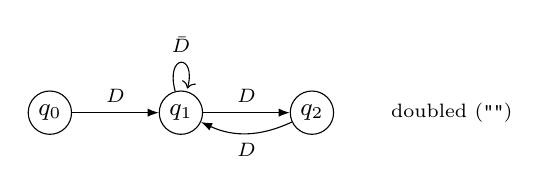
\begin{tikzpicture}[node distance=11mm, font=\small,
  st/.style={draw, circle, inner sep=1pt, minimum size=5.5mm},
  ar/.style={-{Latex[length=1.4mm]}}]
\node[st] (q0) {$q_0$};
\node[st, right=of q0] (q1) {$q_1$};
\node[st, right=of q1] (q2) {$q_2$};
\draw[ar] (q0) -- node[above,font=\scriptsize]{$D$} (q1);
\draw[ar] (q1) edge[loop above] node[font=\scriptsize]{$\bar D$} (q1);
\draw[ar] (q1) -- node[above,font=\scriptsize]{$D$} (q2);
\draw[ar,bend left=25] (q2) to node[below,font=\scriptsize]{$D$} (q1);
\node[right=6mm of q2, font=\scriptsize] {doubled ($\texttt{""}$)};
\end{tikzpicture}
\caption{Masking from the automaton.  A byte is masked iff its transition
consumes it inside a token; this is exact for doubled delimiters, where a
per-state ``inside'' bit is off by one at the closing quote.}
\label{fig:mask}
\end{figure}

\subsection{Cost model}
\label{sec:cost}

Primitives characterize \emph{which} computations are data-parallel; they do not
by themselves yield end-to-end throughput.  For an $n$-byte input producing $k$
tokens, on a discrete accelerator
\[
  T = T_{\mathrm{move\text{-}in}}(n) + T_{\mathrm{compute}}(n,k)
      + T_{\mathrm{move\text{-}out}}(k) + T_{\mathrm{intermediate}} .
\]

\begin{proposition}[Movement bound]
$\Rone$--$\Rseven$ give $T_{\mathrm{compute}} =
O(n\,\mathrm{polylog}\,n / \mathrm{BW}_{\mathrm{gpu}})$ with $O(\log n)$ depth,
independent of $T_{\mathrm{move}}$.  Hence end-to-end throughput $n/T$ is
governed by $\max(T_{\mathrm{compute}}, T_{\mathrm{move}})$; if primitives
materialize $\Theta(n)$ intermediates and results are copied to the host,
$T_{\mathrm{move}}$ dominates and the parallelism of $\SA$ is unobservable.
\end{proposition}

This is why the compiler must also choose a \emph{schedule}: placement (results
stay on device), fusion (compose $\Rone\circ\Rthree\circ\Rfour$ in one pass), and
streaming (chunked pipelining).  We make the schedule explicit in
\S\ref{sec:impl} and measure its effect in \S\ref{sec:eval}.

\section{Implementation}
\label{sec:impl}

The compiler is a header-only C++ library; the CUDA backend is a single header.
A grammar is a C++ type; all lowering happens at compile time, so the generated
scanner is an ordinary templated kernel with no dispatch cost.

\subsection{Front end: shape-free lowering}
\label{sec:frontend}

The front end (\code{include/pars/compile/}) reads only rule definitions:
\begin{enumerate}
  \item \textbf{Recursion analysis.} The rule reference graph is traversed with a
    visited set to compute, per rule, whether it lies on a cycle and how many
    direct self-references it has (cycle glue has none).
  \item \textbf{Automaton.} Each lexical rule body is reified to a regular
    expression in a fixed-capacity arena (no dynamic allocation, so it is
    constant-evaluable by strict front ends such as \textsf{nvcc}) and compiled
    to a DFA by Brzozowski derivatives.  States are canonical derivatives;
    alternatives are normalized by ACI sorting and deduplication, and the
    alphabet is the quotient of $\Sigma$ by membership in every character
    predicate, keeping the DFA tiny even for dense complement predicates.
  \item \textbf{Descriptors.} For each lexical rule we store a \emph{monoid
    descriptor} (\S\ref{sec:backend}).  The unified mask predicate of
    \S\ref{sec:when} decides whether the rule masks at all.
  \item \textbf{Brackets.} A recursive rule is accepted as a well-nested anchor
    only if its top-level definition has exactly the two literal endpoints,
    distinct, with the recursion strictly inside (a conservative, sufficient
    structural criterion); well-nestedness is additionally validated at run time.
  \item \textbf{Diagnostics.} Unsupported recursion or unsupported \code{notp}
    forms are a compile error unless the rule is declared in
    \code{fallback\_rules}.
\end{enumerate}

\subsection{Monoid descriptors}
\label{sec:descriptor}

A descriptor is a small structural value (an NTTP) of one of these kinds:
\begin{itemize}
  \item \textbf{affine}: a delimiter set plus an optional prefix-escape byte
    (executed as $x'=(a\wedge x)\oplus b$);
  \item \textbf{doubled}: a delimiter set (parity on valid input);
  \item \textbf{comment}: a start set and a newline reset;
  \item \textbf{table}: a $\le 8\times 8$ transition table with a
    per-transition mask bit.
\end{itemize}
The kind is read off the DFA; importantly, the execution of \emph{every} kind is
defined by the same automaton table, so a specialization is a performance choice,
not a semantic one.

\subsection{Backends}
\label{sec:backend}

\paragraph{CPU.}
The CPU backend executes descriptors as a per-byte state transform; the running
state is the prefix product (\Rfour).

\paragraph{CUDA.}
The GPU backend packs all descriptors into one 64-bit transform: each descriptor
owns a contiguous range of $4$-bit slots, and we precompute a $256$-entry
per-byte transform table (absolute slot encoding).  Per $32$-byte word we compose
the word transform (each thread), run a \code{thrust} inclusive scan of the
packed transforms, and replay to recover the per-byte state and emit the
per-transition mask.  The scan slot width is \code{total\_states}, and the tables
are staged into shared memory; a compile-time gate rejects
$\code{total\_states}>16$.

\subsection{Schedule}
\label{sec:schedule}

The plan separates compute from movement.  \code{scan\_device} is zero-copy
(device input, device results; only scalar count read-back); \code{scan\_host}
is the only adapter with bulk transfers (pinned, asynchronous), and
\code{scan\_chunk} carries the packed prefix-monoid element and the compaction
offset so a caller can double-buffer chunks across two streams.  The bracket
pairing uses a depth radix sort (\Rsix) rather than a comparison sort.

\section{Evaluation}
\label{sec:eval}

\paragraph{Testbeds.}
We evaluate on two machines, using the same harness and grammars.  The raw
measurements are shared, while figures are rendered separately per
environment.
\begin{itemize}
  \item \textbf{Laptop (4060)}: an Intel i9-13980HX with an NVIDIA RTX~4060
        Laptop GPU (8\,GB GDDR6, \code{sm\_89}, CUDA 13.4, GCC 16), used
        dedicated, on a PCIe~4.0~$\times$8 link.
  \item \textbf{Server (A100)}: a two-socket AMD EPYC~7742 (Zen~2,
        $2\times64$ cores) with an NVIDIA A100-PCIE-40GB (40\,GB HBM2,
        \code{sm\_80}, CUDA 12.6, GCC 10) on a PCIe~4.0~$\times$16 link.
        It is a \emph{shared} login node, so the CPU side is contended.
\end{itemize}
The two machines matter because the GPU and CPU parts of the benchmark scale
with different resources.  The generated scanners run on the GPU; the CPU
baselines (\textsf{simdjson}, \textsf{simdcsv}, \textsf{toml++},
\textsf{pugixml}, \textsf{inih}, \textsf{flex}) run on the host and are bounded
by the host CPU.  We therefore compare each baseline \emph{within a single
environment} only, and we never derive a speedup across machines;
Table~\ref{tab:sota} reports the device numbers for both.

\paragraph{Throughput tiers.}
Each generated scanner is measured at three transport intervals on the
algebra's \Rone--\Rsix axis (\Rone{} classify, \Rtwo$\cdot$\Rfour{} mask+state
scan, \Rthree$\cdot$\Rfive{} compact, \Rsix{} bracket pairing):
\begin{itemize}
  \item \textbf{N1} (\emph{device-resident, no transfer}): the input is uploaded
        once \emph{outside} the timed region and results stay in device memory.
        \textbf{N1a} $=$ \Rone--\Rfive; \textbf{N1b} $=$ \Rone--\Rsix.  This is
        the compute roofline of the generated kernels.
  \item \textbf{N2} (\emph{H2D only}): the input is copied to the device every
        iteration; results stay on device.  This is the interval that matches
        \textsf{cuJSON}'s own Fig.~9 total (H2D $+$ validation $+$ tokenization
        $+$ structure, \emph{no} D2H).
  \item \textbf{N3} (\emph{host boundary, H2D $+$ D2H}): the structural index is
        copied back; \textbf{N3c} is the same boundary with chunked
        double-buffered overlap (the packed prefix-scan carry is threaded across
        chunks).
\end{itemize}
All tiers are \emph{structural}: they stop at \Rsix{} and return a
structural-index-plus-bracket-partners representation, exactly what
\textsf{cuJSON}'s Tokenize$+$Parser and \textsf{simdcsv} produce.  Value
materialisation and queries are a user layer \emph{outside} \Rone--\Rsix{} and
are measured separately (Fig.~\ref{fig:parse}).  We generate inputs of
8\,MB--512\,MB (powers of two).  The device-resident whole-buffer path is
memory-limited on the 8\,GB laptop GPU, so we cap the device-resident scales at
512\,MB; the chunked path (N3c) uses $O(\text{chunk})$ extra memory, the route
\textsf{cuJSON} takes for its 1\,GB datasets~\cite{cujson}.  Before timing we
warm up the process and discard the first iterations, and we report the mean of
$N{=}3$ repetitions (scaling curves) or the median with min--max whiskers
(SOTA bars); \textsf{cuJSON} is averaged over 10 fresh processes, as in its own
harness.

\begin{table*}[t]
\centering\small
\caption{Domain SOTA availability, the output each baseline produces, and the
device-resident \Rone--\Rfive{} throughput (N1a, GB/s, at 512\,MB) on the two
testbeds.  TOML, XML and INI have \emph{no} SIMD/CUDA parser; we use the best
optimized CPU parser.  $^\star$Baselines producing the same output as pars
(a structural index / token stream), hence like-for-like; the others build a
full DOM (or key/value map) and thus do strictly more work.  Device-resident
numbers track the GPU and are comparable across machines; CPU baselines are
not, and are reported per environment.}
\label{tab:sota}
\begin{tabular}{@{}lllrr@{}}
\toprule
Format & SOTA & Baseline (output) & N1a 4060 & N1a A100 \\
\midrule
JSON & simdjson, cuJSON & simdjson (DOM), cuJSON$^\star$ & 16.4 & 40.2 \\
CSV  & simdcsv           & simdcsv (index)$^\star$      & 33.0 & 141.2 \\
TOML & (none)            & toml++ (DOM)                 & 15.0 & 36.2 \\
INI  & (none)            & inih (map)                   & 21.1 & 61.9 \\
XML  & (none)            & pugixml (DOM)                & 17.0 & 34.6 \\
C-like & (none)          & flex (tokens)$^\star$        & 16.5 & 49.3 \\
\bottomrule
\end{tabular}
\end{table*}

\paragraph{Scaling.}
Figure~\ref{fig:scaling} shows throughput versus input size, one facet per
format.  The three pars series are the transport tiers: \textbf{N1} (device,
no transfer), \textbf{N2} (H2D only) and \textbf{N3c} (host boundary, chunked).
The device numbers (N1) rise with the working set and then track the GPU memory
bandwidth; the host-boundary numbers (N3c) start low (dominated by fixed
launch/transfer overhead), rise as the overhead is amortized, and then plateau.
The vertical gap between N1, N2 and N3c is exactly the cost of moving the input
and the result, which is why the same generated scanner can look an order of
magnitude apart depending on the interval.

\paragraph{Transport, and the \textsf{cuJSON} interval.}
We report \textsf{cuJSON} at \emph{its own} Fig.~9 interval, i.e.\ excluding D2H.
This matters: its total includes H2D $+$ validation $+$ tokenization $+$
structure and the result copy-back, and the copy-back is \emph{not} overlapped,
so adding D2H cuts its throughput roughly in half to two thirds at 512\,MB.
The matched pars interval is therefore \textbf{N2} (H2D $+$ \Rone--\Rsix, no
D2H), not N1 (which does not even pay H2D) and not N3 (which adds D2H).  At that
interval \textsf{cuJSON} remains the strongest structural JSON parser; N3c, which
additionally overlaps the copy-back, is the comparison at the host boundary.
Reporting \textsf{cuJSON} with D2H while comparing against a no-D2H pars tier
(and vice versa) would be an interval mismatch, so we always pair the same
boundary.

\paragraph{Host-boundary CSV versus \textsf{simdcsv}, and why it is
environment-dependent.}
The end-to-end (N3c) CSV number moves $n + k\cdot w$ bytes over PCIe
($k$ separators, $w{=}4$ bytes each, i.e.\ $\sim$1.5$n$), so its ceiling is
$BW\cdot n/(n+k\cdot w)$, \emph{not} the raw link bandwidth: even with perfect
overlap the input and the result share the link, and in N3c the D2H copy is a
serial tail after the chunk loop.  The two testbeds land on opposite sides of
this crossover.  On the laptop the host-boundary path is PCIe-bound
(7.5\,GB/s for N3c vs.\ 9.1\,GB/s for \textsf{simdcsv}, which streams from CPU
DRAM) and stays \emph{below} \textsf{simdcsv}; on the A100 node
\textsf{simdcsv} is limited by the older, shared server CPU (6.0\,GB/s) while
N3c reaches 12.7\,GB/s, so the host-boundary path \emph{wins}.  The
device-resident N1 number is far above \textsf{simdcsv} on both (33 vs.\
9.1\,GB/s on the laptop, 141 vs.\ 6.0\,GB/s on the server), and is where the
generated scanner's headroom actually lives.

\paragraph{Cross-environment anomalies.}
\begin{itemize}
  \item \textbf{CPU baselines are host-bound.}  The A100 node's EPYC~7742 is
        roughly 1.5--2$\times$ slower per core than the laptop's i9-13980HX, so
        \textsf{simdjson} ($1.7\to1.0$), \textsf{simdcsv} ($9.1\to6.0$),
        \textsf{flex} ($0.68\to0.33$), \textsf{inih} ($0.32\to0.15$) and
        \textsf{toml++} ($0.044\to0.021$) all \emph{drop} on the server
        (GB/s at 512\,MB) despite its far faster GPU.  The exception is
        \textsf{pugixml} ($0.44\to0.57$\,GB/s): its DOM construction is
        allocation- and memory-bound and benefits from the server's larger
        caches and more memory channels, so the CPU ranking is \emph{not}
        uniform.  Ratios between a CPU baseline and a generated GPU scanner are
        therefore meaningful only within one environment; we never quote a
        cross-machine speedup.
  \item \textbf{GPU tiers track the GPU, not the host.}  Device-resident N1a at
        512\,MB is $2$--$4\times$ higher on the A100 (CSV 33$\to$141, JSON
        16$\to$40, INI 21$\to$62\,GB/s), tracking HBM bandwidth and SM count
        rather than the grammar.  The GPU baselines move the same way:
        \textsf{cuJSON} rises $5.2\to10.9$\,GB/s, since the laptop's
        $\times$8 link is the narrower one.
  \item \textbf{Shared node $\Rightarrow$ dispersion.}  The A100 node is a
        shared login node, so its run-to-run spread is larger (visible in the
        min--max whiskers); we warm up before timing and prefer medians for the
        SOTA comparison, means for the scaling trend.
  \item \textbf{Full parse can lose even when stage-1 wins.}  For JSON the
        end-to-end parse (Fig.~\ref{fig:parse}) adds a \emph{host} semantic
        layer that decodes values and builds a DOM; it is sequential and not
        generated, so pars trails \textsf{simdjson}'s optimized DOM tape by
        $\sim$2.4$\times$ even though its stage-1 is far faster.  This is a
        stage-2 cost, not a scanning cost.
\end{itemize}

\begin{figure*}[t]
\centering
\paperfig{fig_scaling}{Throughput vs input size}
\caption{Throughput vs.\ input size (log--log axes; mean of $N$ runs).  The pars
tiers separate the transport cost: \textbf{N1} is device-resident ($R1$--$R5$,
no transfer), \textbf{N2} adds H2D only (results stay on device), and
\textbf{N3} is the host boundary including D2H (the chunked-overlap variant
$N3c$).  Device stage-1 rises with the working set and tracks GPU memory
bandwidth; the host-boundary path starts low (fixed launch/transfer cost) and
then plateaus at the PCIe limit ($1.5n$ bytes moved).  For CSV the host path
stays below \textsf{simdcsv} on the laptop but surpasses it on the server, where
the CPU baseline is the bottleneck.  \textsf{cuJSON} is shown at its own Fig.~9
interval (H2D $+$ validation $+$ tokenization $+$ structure, \emph{excluding}
D2H).}
\label{fig:scaling}
\end{figure*}

\begin{figure}[t]
\centering
\paperfig{fig_stages}{Per-stage GPU time}
\caption{Per-stage GPU time on the \Rone--\Rsix{} axis (512\,MB).  The
mask$+$scan stage (\Rtwo$\cdot$\Rfour) dominates where the descriptor scan is
generic (multi-mode/table); bracket pairing (\Rsix) dominates bracket-heavy
JSON.}
\label{fig:stages}
\end{figure}

\paragraph{End-to-end parse, matched per format.}
The tiers above are scoped to \Rone--\Rsix, so Figure~\ref{fig:parse} matches
each format at the interval its baseline actually covers.  For TOML, XML and INI
we add a host post-\Rsix{} layer on the same hook: \code{replay} drives a user
parser that decodes values ($M$) and builds a map or tag tree ($D$), all
format-specific and living outside \code{include/}; we validate that the
resulting counts match the baselines exactly (sections, entries, elements,
attributes).  Both sides then perform a \emph{full parse}; for TOML, INI and XML
pars is ahead of (or at parity with) the CPU DOM parsers.  For JSON the
like-for-like baseline is
\textsf{simdjson}'s DOM parse; pars' GPU stage-1 is fast but the host DOM hook
dominates, so pars trails there (a stage-2 gap, not a scanner gap).
\textsf{cuJSON} is a GPU parser whose output is a \emph{structural index}
(\Rone--\Rsix), not a DOM, so it is compared at the structural N2 interval
(Fig.~\ref{fig:scaling}), never as a full parse.

\begin{figure}[t]
\centering
\paperfig{fig_parse}{End-to-end comparison, matched per format}
\caption{End-to-end comparison at 512\,MB, matched per format (log scale).
JSON is compared at the \emph{structural} interval (pars N2 $=$
$T_{\mathrm{in}}+$R1--R6, no D2H, vs \textsf{cuJSON}'s Fig.~9 total); TOML/INI/XML
are \emph{full parses} (pars $=$ GPU \Rone--\Rsix{} $+$ host $M{+}D$ vs the DOM
parser of each format), where the host semantic layer, not the scanner,
dominates.}
\label{fig:parse}
\end{figure}

\paragraph{SOTA comparison and fairness.}
Figure~\ref{fig:sota} compares the generated stage-1 scanner (N1a) with each
format's baseline at 512\,MB.  The comparison is \emph{not} end-to-end
equivalent: pars returns a structural index (positions of delimiters, quotes and
brackets), whereas \textsf{simdjson}, \textsf{toml++}, \textsf{pugixml} and
\textsf{inih} additionally materialize a DOM or key/value map.  We therefore
report stage-1 throughput as \emph{headroom} for the data-parallel scan, not as
a full-parse speedup, and separate the like-for-like baselines
($^\star$ in Table~\ref{tab:sota}): \textsf{simdcsv} computes exactly the same
structural index as pars CSV, \textsf{flex} is a pure tokenizer, and
\textsf{cuJSON} is the GPU structural JSON parser.  The large gaps on
TOML/INI/XML reflect the extra DOM-building work those baselines perform; they
bound the scanning cost rather than demonstrate an end-to-end win, which
Fig.~\ref{fig:parse} addresses directly.

\begin{figure}[t]
\centering
\paperfig{fig_sota}{Stage-1 vs SOTA}
\caption{Device stage-1 vs.\ chunked host path vs.\ the strongest implementation
of each format at 512\,MB (log scale, min--max whiskers over repeats).  pars
(and \textsf{simdcsv}, \textsf{flex}, \textsf{cuJSON}) return a structural or
token index; \textsf{simdjson}, \textsf{toml++}, \textsf{pugixml} and
\textsf{inih} build a full DOM, so those bars bound the scanning cost rather
than an end-to-end comparison.}
\label{fig:sota}
\end{figure}

\paragraph{Correctness.}
Every generated scanner is validated against a CPU implementation on the full
input and on random adversarial inputs (unterminated strings, doubled quotes,
star runs in block comments, comments to EOF); the format-specific full-parse
hooks are validated so that their counts match the baselines.  The GPU and CPU
backends are cross-checked index-for-index.

\paragraph{XML and YAML.}
XML is currently a \emph{stage-1} scanner: it masks attribute
values and derives the structural set $\{<,>,/,=,?,!\}$, but does not model tag
nesting; full XML needs the visibly-pushdown call/return extension for named
tags.  YAML needs an indentation primitive (an all-nearest-smaller-value stack);
it is not supported yet.  Both are natural next milestones.

\section{Related Work}
\label{sec:related}

The algebraic components of $\SA$ are classical.  Parallel prefix is
Blelloch's scan~\cite{blelloch}, with the classic
Ladner--Fischer~\cite{ladnerfischer} and Hillis--Steele~\cite{hillissteele}
constructions and GPU scan/compaction primitives~\cite{sengupta}; that a finite
automaton is a transformation monoid is
textbook~\cite{eilenberg,hopcroftullman}, and regular expressions are decided by
derivatives~\cite{brzozowski}; the scan lemma and promotion come from the
Bird--Meertens theory of lists~\cite{birdlists,birddemoor,meertens}; the
well-nested reduction is \textsf{cuJSON}'s stack-free
matching~\cite{cujson}; the bracket/stack monoid is Levien's \emph{Stack
Monoid}~\cite{stackmonoid}; parallel bracket matching / tree contraction is
classical~\cite{baronvishkin,millerreif}; and well-nested recursion is precisely
the visibly-pushdown class of Alur and Madhusudan~\cite{alur}.  Our stance that
these are instances of one structured parallel pattern is in the tradition of
algorithmic skeletons~\cite{cole} and of algebraic treatments of parsing
(semiring parsing~\cite{goodman}).  We do not claim the algebra itself.

Our claim is its \emph{systematization into a compiler}.  \textsf{simdjson}
\cite{simdjson} and \textsf{simdcsv} \cite{simdcsv} hand-write the primitives
for one format each; \textsf{cuJSON} \cite{cujson} and \textsf{GpJSON}
\cite{gpjson} do so on the GPU; \textsf{Mison} \cite{mison},
\textsf{Sparser} \cite{sparser} and \textsf{Pison} \cite{pison} optimize JSON
ingestion in data systems.  None exposes a grammar-to-parallel-parser
derivation, and none distinguishes compute parallelism from data movement as a
compiler concern.  XML and YAML parsers such as \textsf{pugixml}
\cite{pugixml} and \textsf{rapidyaml} remain optimized sequential parsers; to
our knowledge no SIMD or GPU parser exists for TOML, XML, YAML or INI, which is
exactly the setting where a generator has no hand-written baseline to match.
On the scanner side, the classical generators \textsf{lex}~\cite{lex} and
\textsf{re2c}~\cite{re2c} compile regular expressions to a table-driven DFA with
longest-match semantics, and \textsf{Hyperscan}~\cite{hyperscan} vectorizes
multi-pattern matching, but none exposes the transformation-monoid scan used
here.  General-value parsing (CYK/Earley~\cite{earley}, or Valiant's reduction to
Boolean matrix multiplication~\cite{valiant}) is parallelizable in theory but
not competitive in practice, and we do not target it.

\section{Conclusion}
\label{sec:conclusion}

We presented the scan algebra $\SA$, a rewrite system that turns a naive branch program
into branchless masked data flow over a transformation monoid, and a compiler
that lowers a grammar to a data-parallel scanner using $\SA$.  The algebra is
classical; the contribution is making the derivation mechanical and explicit,
including the difference between compute parallelism and data movement.  The
generated device-resident scanners match hand-written SOTA where one exists
(CSV, JSON) and run far ahead of the best CPU parsers for formats that no one
has vectorized (TOML, INI, C-like); adding host-boundary data movement, not
compute, is what decides whether that lead survives end to end.
Extending the recursion primitives to indentation (YAML) and
named-tag nesting (XML) is the natural next step, and would let the generator
claim the formats where it has the most to offer.

The compiler, grammars, and benchmarks are open source.


\bibliographystyle{ACM-Reference-Format}
\bibliography{refs}

\end{document}
